% !TEX root = scheduler.tex
\section{Design of the Scheduler}\label{sec:design}
In this section we present an overview of the components in the proposed \sys{} scheduler.
%, and its various components. the \textit{Policy Enforcer} and the \textit{Learning Agent}. 

\subsection{Scheduler Architecture Overview}\label{ssec:scheduler-arch}
Figure~\ref{fig:scheduler-architecture} shows the architecture of the \sys{} scheduler.
We first describe the \textit{Query Manager}. 
Each query in the system has its own private instance of the Query Manager.
It manages the progress of the query that it owns.
The Query Manager maintains the query plan DAG and a data structure called
the \textit{Work Order Container} to track all the work orders that are ready for
scheduling. 
Recall from Section~\ref{sec:background}, a description of the work 
carried out on a block of data is a \textit{work order}. 

\begin{figure}
	\centering
	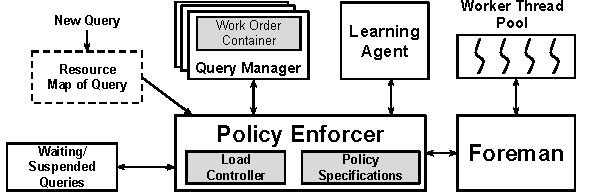
\includegraphics[width=\columnwidth]{figures/Scheduler-Architecture.pdf}
	\vspace*{-1.5em}
	\caption{Overview of the scheduler}
	\label{fig:scheduler-architecture}
	\vspace*{-1.5em}
\end{figure}

The Query Manager generates schedulable work orders for each active operator node
in the DAG, and stores them in the Work Order Container.
It also runs the core algorithm to determine when to activate nodes in the DAG. 
Details about work orders are presented in Section~\ref{ssec:workorders}.
%and Section~\ref{sssec:dag-traversal-example}.
The Query Manager DAG node processing algorithm is described in
Section~\ref{ssec:DAG-algo}. 

An important component of the system is the \textit{Policy Enforcer}. 
It selects a query among all the concurrent queries, and schedules its work order for execution. 
This in essence is a scheduling decision, and is taken based on a high-level policy provided to the system.
The policy is described in \textit{Policy Specifications}, which is an
abstraction that governs how resources are shared among concurrent queries. 

A two-way communication happens between the Policy Enforcer and the various Query Managers.
The Policy Enforcer requests a Query Manager to return a certain number of work orders from the query that it manages.
These work orders are then dispatched for execution by the Policy Enforcer. 
The Policy Enforcer communicates with the Query Manager upon every work order
completion, so that the Query Manager can then decide if new nodes in the DAG
can be activated, and if existing nodes can be marked as completed.
A detailed description of the Policy Enforcer is present in Section~\ref{ssec:policy-enforcer}. 

The Policy Enforcer contains a \textit{Load Controller} module, which is
responsible for ensuring that the system has enough resources to meet the
demands.
A new query in the system presents its resource requirements in the form of a
\textit{Resource Map} to the Load Controller.
The Resource Map describes the estimated resource requirements of the query
during its lifetime. 
An example Resource Map is shown below:%in Table~\ref{table:sample-resource-map}.
\begin{lstlisting}[language=python, 
								   basicstyle=\ttfamily\small, 
								   showstringspaces=false,
								   keywordstyle=\color{bondiblue}\bfseries, 
								   emph={CPU, Memory}, 
								   emphstyle=\color{cardinal}\bfseries]
CPU:    {min: 1 Core, max: 20 Cores}
Memory: {min: 20 MB,  max: 100 MB}
\end{lstlisting}
\vspace{-0.5em}
%\begin{table}[h]
%	\centering
%	\begin{tabular}{|p{0.2\columnwidth}|p{0.3\columnwidth}|p{0.3\columnwidth}|}
%		\hline
%		\textbf{Resource} & \textbf{Estimated min requirement} & \textbf{Estimated max requirement} \\ \hline
%		CPU & 1 Core & 20 Cores \\ \hline
%		Memory & 20 MB & 100 MB \\ \hline
%	\end{tabular}
%	\vspace{0.5em}
%	\caption{A sample resource map}
%	\label{table:sample-resource-map}
%	\vspace{-1.5em}
%\end{table}

This Resource Map states that the query can use 1 to 20 cores (i.e. specifies the range of intra-operator parallelism) and is estimated to require a minimum of 20 MB of memory to run, and an estimated 100 MB of memory in the worst case.
%The estimates provided in Resource Map can come from the query optimizer or some
%other mechanism, which is irrelevant to the scheduler.
The Load Controller determines the action to be taken with the new query. 
If enough resources are available, it admits the query.
If the system can potentially thrash due to the admission of the new query, it
can take a number of decisions, including wait-listing the query or
suspending one or more queries that are currently running to free up resources for the new query.
The Policy Enforcer maintains queues for wait-listed and suspended queries as shown in Figure~\ref{fig:scheduler-architecture}.
The Load Controller is described in detail in Section~\ref{ssec:load-control-mech}.

%A new query in the form of a DAG from the optimizer is sent to the Policy Enforcer.
%It decides when to activate or deactivate an entire query,
%as a means to \textit{admission control}. 
%The current admission control is simple and limits the number of concurrent 
%queries to a pre-defined number.  
%(It is easy to extend this component to examine factors such as buffer pool 
%swapping activity or cache miss rates to realize a different load control policy.)

The Policy Enforcer works with another module called the \textit{Learning Agent}. 
Execution statistics of completed work orders are passed from the Policy Enforcer to the Learning Agent.
This component uses a simple learning-based method to predict the time to 
complete future work orders using the execution times of finished work orders. 
Such predictions form the basis for the Policy Enforcer's decisions regarding scheduling the next set of work orders. 

%Work orders that are ready to execute are sent to a \textit{Foreman} module. 
%The Foreman simply acts as a link between the overall scheduler and a pool of 
%worker threads. 
The \textit{Foreman} module acts as a link between the Policy Enforcer and a pool of worker threads. 
It receives work orders that are ready for execution from the Policy Enforcer, and dispatches them to the worker threads. 
The Foreman can monitor the number of pending work orders for each worker, and 
use that information for load-balancing in work order dispatch.
When a worker completes executing a single work order, it sends a completion message 
to the Foreman.
This message contains statistics about the work order execution, which the Foreman passes on to the Policy Enforcer. 
During a work order execution, output data may be created (in blocks in the buffer pool). 
When an output data block is filled, the worker thread sends a message to the 
Foreman informing it about the filled block. 
The Foreman then forwards this information to the Policy Enforcer, 
which in turn communicates this information to the Query Manager. 
The Query Manager may then create a new work order based on this information;
e.g. if this block should be pipelined to another operator in the query plan.
%Next, we describe \sys{} schedulers's thread organization model. 

\subsection{Thread Model}\label{ssec:thread}
\sys{} currently runs as a single server process, with mutiple user-space threads. 
There are two kinds of threads. 
There is one \textit{Scheduler} thread, and a pool of \textit{Worker} threads. 
All the components in 
Figure~\ref{fig:scheduler-architecture} except the worker thread pool run in the 
scheduler thread. 
In the current implementation, all threads are spun upfront when the database server 
process is instantiated, and stay alive until the server process terminates.

The threads use the same address space and use shared-memory semantics for data 
access. 
In fact the buffer pool is stored in shared memory, which is accessible by all the threads. 
%Each worker thread is typically pinned to a CPU core. 
%Such pinning avoids costs incurred when a thread migrates from one CPU core to another, which results in loss of data and instruction cache locality. 

Every worker thread receives a work order from the Foreman, executes it and then waits for 
the next work order.
In order to minimize worker's idle time, typically each worker is issued multiple work 
orders at any given time. 
%When a work order is sent to a worker thread, it executes the work order.
 %the worker thread simply invokes %the appropriate \verb|execute()| method (described in~\ref{ssec:workorders}). 
Thread-safe queues are used to communicate between the threads.
%The communication happens through light-weight messages from the sender to the receiver thread, which is internally implemented as placing a message object on the receiver's queue. 
%A receiver reads messages from its queue. 
%A thread (and its queue) is uniquely identified by its thread ID. 

%The thread communication infrastructure also implements additional features 
%like the ability to query the lengths of any queue in the system, and cancellation 
%of an unread message. 
%For simplicity, we omit discussion of these aspects. 

\subsection{Work Orders}\label{ssec:workorders}
Work done for executing a query in \sys{} is split into multiple \textit{work 
orders}, as highlighted in Section~\ref{sec:background}. 
A work order contains all the information that is needed to process tuples in a given 
data block. 
A work order encapsulates the relational operator that is being applied, the relevant 
input relation(s), location of the input data block, any predicate(s) to be 
applied on the tuples in the input block, and descriptors to other run-time 
structures (such as hash tables).
%The input data location is specified in terms of a unique storage block ID, a join hash table identifier, or an aggregation hash table identifier. 
%In NUMA settings, a work order can also provide a preferred site for execution in the 
%form of a NUMA socket ID. 
%The scheduler then uses this information to make a 
%\textit{data-locality aware} scheduling decision. \reminder{Should we remove NUMA 
%because there are no experiments?}

Consider the following full table scan query to illustrate the work order concept:

\begin{lstlisting}[language=SQL, 
basicstyle=\ttfamily\small, 
showstringspaces=false,
keywordstyle=\color{cardinal}\bfseries, 
emph={San,Diego}, 
emphstyle=\color{bondiblue}\bfseries]
SELECT name FROM Employee WHERE city=`San Diego'
\end{lstlisting}	
\vspace{-0.4em}

The plan for this query has a simple \textit{selection} operator.  
For the selection operator, the number of work orders is same as the number of input blocks in the \verb+Employee+ table. 
Each selection work order contains the following information:
\begin{itemize}
\itemsep0.1em
\item {Relation: \verb+Employee+, attribute: \verb|name|}
\item {Predicate: \lstinline[language=SQL, 
                                   basicstyle=\ttfamily\small, 
                                   keywordstyle=\color{cardinal} \bfseries,
                                   emph={San,Diego}, 
                                   emphstyle=\color{bondiblue}\bfseries]|city=`San Diego'|}
\item {The unique ID of an input block from the \verb+Employee+ table}
\end{itemize}

The work orders for a join operation %(illustrated below) 
are slightly more complicated. 
For example, a \textit{probe work order},  contains the unique ID of the probe 
block, 
%(as described in Section~\ref{ssec:storage-manager}, a hash table is stored in a block in the buffer pool), build and probe relations, 
a pointer to the hash table, the projected attributes, and the join predicate.
%Each operator algorithm (e.g. a scan or the build/probe phase of a hash-join) 
%in the system has a C++ class that is derived from 
%a root abstract base class that has a virtual method called \verb|execute()|.
%Executing a work order simply involves calling the \verb|execute()| method 
%on the appropriate operator algorithm C++ class object. 

\subsection{DAG Traversal Algorithm}\label{ssec:DAG-algo}
The Query Manager is presented with a DAG for each query, where each
node in the DAG represents a relational operator primitive.
The edges in the DAG are annotated with whether the 
\textit{consumer} operator is blocked on the output produced 
by the \textit{producer} operator, or whether data pipelining is
allowed between two adjacent operators. 

Consider a sample join query and its DAG showed in Figure~\ref{fig:dag}.
The solid arrows in the DAG correspond to ``blocking'' dependencies,
and the dashed arrows indicate pipeline-able/non-blocking dependencies. 
To execute this query we need to select tuples from the \verb+ddate+ 
table, stream them to a hash table, which can then be probed by tuples that are 
created by the selection operator on the \verb+lineorder+ table. %(i.e. match the predicate on that table). 
The output of the probe hash operation can be sent to the print operator, which
displays the result. % tuples. 
Note that the ``drop hash'' operator is used to drop the hash table, but only 
after the ``probe hash'' operation is complete. 
Similarly, the other drop operators indicate when intermediate data can be deleted. 

\begin{algorithm}[t]
%	\algsetup{linenosize=\tiny}
%  \scriptsize
	\caption{DAG Traversal}
	\begin{algorithmic}[1]
		\State G = \{V, E\}
		\State activeEdges = \{e $\in$ E $|$ e.isNotPipelineBreaking()\}
		\label{alg:pipelining}
		\State inactiveEdges = \{e $\in$ E $|$ e.isPipelineBreaking()\}
		\State completedNodes = \{\}
		
		\For {v $\in$ V}:
			\If {v.allIncomingEdgesActive()}
				\State v.active = True
			\Else
				\State v.active = False
			\EndIf
		\EndFor
		
		\While {completedNodes.size() $<$ V.size()}
		\For {v $\in$ V -- completedNodes}
		\If {v.allIncomingEdgesActive()}
			\State v.active = True \label{alg:depMet}
		\EndIf
		\If {v.active}
		\State v.getAllNewWorkOrders() \label{alg:getWork}
		\If {v.finishedGeneratingWorkOrders()} \label{alg:finishGenWork}
		\State completedNodes.add(v) \label{alg:nodeComplete}
		\For {outEdge $\in$ v.outgoingEdges()}
		\State activeEdges.add(outEdge)\label{alg:outEdgesActive}
		\EndFor
		\EndIf
		\EndIf
		\EndFor	
		\EndWhile
	\end{algorithmic}
	\label{alg:dag-traversal}
\end{algorithm}

The Query Manager uses a DAG Traversal algorithm (cf. Algorithm~\ref{alg:dag-traversal}) to process the DAG, which essentially is an iterative graph traversal method. 
The algorithm simply finds nodes in the DAG that have all their dependencies met, and marks such nodes as ``active'' (line~\ref{alg:depMet}).
Work orders are requested and scheduled for all active nodes (line~\ref{alg:getWork}), and 
the completion of work orders is monitored. 
Operators are stateful and they produce work orders when they have the necessary data.
The work order generation stops (line~\ref{alg:finishGenWork}) when the operators no longer have any input to produce additional work orders.
When no more work orders can be generated for a node, that node is marked as 
``completed'' (line~\ref{alg:nodeComplete}). 
When a node is marked as completed, all outgoing blocking edges (the solid lines 
in Figure~\ref{fig:dag}) are ``activated'' (line~\ref{alg:outEdgesActive}). 
Pipelining is achieved as all non-blocking edges (dotted lines in 
Figure~\ref{fig:dag}) are marked as active upfront (line~\ref{alg:pipelining}).
The query is deemed as completed when all nodes are marked as ``completed.''

\begin{figure}[h]
	\centering
	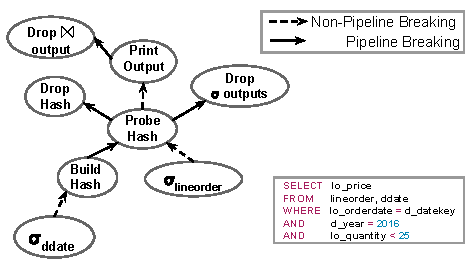
\includegraphics[width=\columnwidth]{figures/QueryPlan.pdf}
	\vspace*{-2em}
	\caption{A join query and its DAG}
	\label{fig:dag}
%	\vspace*{-1.5em}
\end{figure}

% Note(harshad) - The DAG traversal example seems to be taking lots of space and can be omitted, as it diverts the attention away from the meat of the paper. 
%\subsubsection{DAG Traversal Example}\label{sssec:dag-traversal-example}
%To illustrate the execution of the scheduler algorithm, consider the 
%DAG shown in Figure~\ref{fig:dag}.
%Initially, only the two selection relational operators (shown in the DAG using
%the symbol $\sigma$) are \textit{schedulable}.\footnote{Initially, the print 
%operator is \textit{active} too, but as there's no input available, it can't
%produce any work order.}
%So, the Query Manager generates work orders for these operators. 
%In this case, there is one work order for each input block in each of the two
%input relations.\footnote{To avoid both select operators from being co-scheduled
%concurrently, a dependency link can be created between these two operators.
%Thus, work on the select operator on the $\mathtt{lineorder}$ table is started
%only after the select operator on the $\mathtt{ddate}$ table has completed. 
%Such decisions are made by the optimizer.}
%
%The Foreman assigns these work orders to the available worker threads. 
%The worker threads execute the operations specified in the work orders. 
%Note that given the independent block design (see Section~\ref{ssec:storage-manager}) 
%it is possible that two work orders on the same table may invoke different code paths. 
%For example one block on the \verb+ddate+ table may have an index sub-block on 
%the \verb+d_year+ attribute, and this index may be chosen to evaluate the tuples 
%in that block. 
%Another block on that same \verb+ddate+ table may not have any indices, and so 
%the selection operation for tuples in that second sub-block may resort to a simple scan. 
%In addition, the operator algorithm may choose to make a local decision on which 
%access plan to use. 
%So, e.g. even if each data block in the \verb+ddate+ table has an index 
%of the \verb+d_year+ attribute some work orders may use the index and others may 
%not. (The optimization algorithm for making these local decisions is beyond the 
%scope of this paper.)
%Essentially, the scheduler is largely oblivious to how the work orders are executed 
%and there is no global recipe that is imposed on the work orders that correspond 
%to a node in the DAG.
%
%Work orders may produce output data that are stored in blocks in the buffer pool. 
%In the case of the query in Figure~\ref{fig:dag}, the selection work orders on the \verb+ddate+
%table insert the selected tuples into data blocks that correspond to a new 
%temporary table. 
%%(the execution of the work orders is vectorized for efficiency). 
%These data blocks are pipelined to the next stage.\footnote{There is a 
%mechanism to allow multiple concurrent work orders from the same
%operator in the DAG to insert into a common output/temporary data
%block to avoid block internal fragmentation, and to facilitate early 
%pipelining. We omit these details.}
%In other words, as soon as there is a full block of tuples from applying the 
%selection operator on the \verb|ddate| table, a work order is created for the 
%\textit{build hash} operator. (Notice that the edge connecting the selection
%operator and the build hash operator permits data pipelining.)
%
%To begin the probe phase of the hash join, the building of the hash table must be 
%complete, as there is a pipeline-breaking dependency between the probe operator 
%and the build operator. 
%Thus, the DAG traversal algorithm only marks the probe hash operator node as 
%active when the build hash operator has completed. 
%Results from probing the hash table can be immediately pipelined to the print 
%operator.
%The drop operators ensure that intermediate data is dropped before the query is 
%deemed to have completed. 

\subsection{Policy Enforcer}\label{ssec:policy-enforcer}
The Policy Enforcer applies a high level policy for resource allocation among concurrent queries. 
It uses a probabilistic-framework to select work orders from a pool of work orders 
belonging to different concurrent queries for scheduling. 
The Policy Enforcer assigns a probability to each active query, which indicates the likelihood of a work order from that query getting scheduled for execution in the near future. 
The probability-based work order selection strategy brings powerful control to the scheduler through a single parameter -- i.e. by controlling the probability 
setting, the scheduler can control the resource sharing among concurrent queries. 
%A work order from a query with higher probability is more likely to get scheduled 
%than a work order from a query with lower probability. 

The challenge in designing the policy enforcer lies in transforming the policy specifications to a set of probabilities. 
A critical piece that we use in such transformations is the prediction of work order 
execution times for the concurrent queries, which is done by the Learning Agent described in Section~\ref{ssec:learning}. %and depicted in Figure~\ref{fig:scheduler-cycle}.
In the remainder of this section, we provide an intuition for deriving probability values from the work order execution times. 
A formal model for the probability computations for different policies is presented in Section~\ref{sec:policy}.

\begin{figure}[]
	\centering
	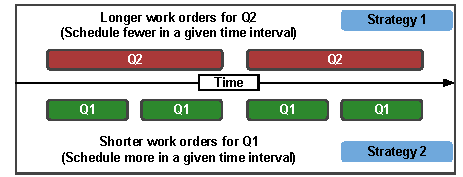
\includegraphics[width=\columnwidth]{figures/Probability-explanation.pdf}
	\vspace{-2em}
	\caption{Scheduling queries having different work order execution times for the fair policy. The solid boxes with $Q_{i}$ depicts the lifetime of a work order from the Query $Q_{i}$.}
	\label{fig:probability-explanation}
	%	\vspace{-1.5em}
\end{figure}

We now motivate the probabilistic approach used by the Policy Enforcer with an example.
Consider a single CPU core and two concurrent queries $q_{1}$ and $q_{2}$. 
(The idea can be extended to multi-cores and more than two queries.)
Initially, we assume perfect knowledge of the execution times of work orders of the queries. 
Later, we will relax this assumption. 

Let us assume that as per the policy specifications, in a given time interval, the CPU resources should be shared equally. 
Suppose that work orders for $q_{1}$ take less time to execute than work orders for 
$q_{2}$, as shown in Figure~\ref{fig:probability-explanation}.
As the Policy Enforcer aims to allocate equal share of the CPU to $q_1$ and $q_2$, a simple strategy can be to schedule proportionally more work orders of $q_{1}$  than those of $q_{2}$, in a given time window. 
The number of scheduled work orders is inversely related to the work order execution 
time. 
This proportion can be determined by the probabilities $pb_{1}$ and $pb_{2}$ for queries $q_1$ and $q_2$, respectively.
The probability $pb_i$ is the likelihood of the scheduler scheduling next work order from query $i$. 
The probability is assigned by the Policy Enforcer to each active query in the system.
Note that, $pb_{1} > pb_{2}$ and $pb_{1} + pb_{2} = 1$.

%Such strategy will result in similar \textit{CPU occupancy} with respect to time 
%for both the queries, thereby fairly sharing the CPU resource in a given time 
%frame.  If the policy enforcer keeps scheduling the work orders similarly for the rest of 
%the  workload execution, it is easy to see that the queries will share the CPU 
%\textit{fairly}, as demanded by the policy. 

Notice that the Policy Enforcer is not concerned with the complexities of the operators in the query DAGs. 
It simply maintains the probability associated with each active query which is determined by the query's %predicted 
work order execution times.

The Policy Enforcer can also function with workloads that consist of queries categorized in multiple classes, where each class has a different level of ``importance'' or ``priority''. 
The policy specifies that the resource allocation to a query class must simply be in accordance to its importance, i.e. queries in a more important class should collectively get a higher share of the resources, and vice versa.
In such scenarios, the Policy Enforcer splits its work order selection strategy in two steps - selection of a query class and subsequent selection of a 
query within the chosen query class.
Intuitively, the Policy Enforcer should assign higher probability to the more 
important class and lower probability to the less important class.

Once a query class is chosen, the Policy Enforcer must pick a query from the chosen class. 
Each query class can specify an optional intra-class resource allocation sub-policy. 
By default, all queries within a class are treated equally.
Thus, the probability-based paradigm can be used to control both inter and intra-class resource allocations.

There could be many reasons for categorizing queries in classes, including the need to associate some form of urgency (e.g. interactive vs batch queries), or marking the importance of the query source 
(e.g. the position of the query submitter in an organizational hierarchy). 
In addition, the resource allocations across different classes can also be chosen based on various scales, such as linear or exponential scale allocations based on the class number. 
An attractive feature of the Policy Enforcer is that it can be easily configured for use in a variety of ways.
Under the covers, the Policy Enforcer simply maps each class to a collective class probability value, and then maps each query in each class to another probability. 
Once these probabilities are calculated, the remaining mechanisms simply use them to appropriately allocate resources to achieve the desired policy goal.

To summarize, the Policy Enforcer assigns a probability value to each active query in the system. 
The scheduling decisions are taken based on these probabilities. 
We also saw the connection between the probability value and the execution time of future work order, with fair policy as a case in point. 
However this raises some questions: How do we know the future execution time of a work order? 
%Second, what happens if the future execution time of work orders keep changing? 
Why should we compute the probability using future work order execution times instead of assigning fixed probabilities to queries?
We answer these questions by introducing a Learning agent module in the next section. 
 
%In the beginning of a workload execution, the Policy Enforcer uses some default 
%probability values until the Learning Agent collects enough data so as to make a prediction. 
\subsection{Learning Agent}\label{ssec:learning}
The Learning Agent module is responsible for predicting the execution times of the future work orders for a given query. 
It gathers the history of executed work orders of a query and applies a prediction model on such a history to estimate the execution time of a future work order.
This predicted execution time is used to compute the probability assigned to each query (cf. Section~\ref{sec:policy} for probability derivations).  
%The Learning agent also helps us relax our earlier assumption, about knowledge of execution times of the future work orders for the queries. 
%In a real implementation, such information is not available.
%To get around this issue, we incorporate a Learning Agent module, described in the next section. 
%It predicts the execution time of future work orders, using a learning methodology. 
%Such predicted execution times are used to compute the probabilities assigned to the queries.

%In this section we describe the Learning Agent module in the scheduler. 
%As described in Section~\ref{ssec:policy-enforcer}, the Learning Agent converts predicted execution times of future work orders to probabilities, which are used for the scheduling decisions.
One might question the need of the Learning Agent and instead consider assigning a fixed probability value to each query (say $1/N$, with $N$ queries in the fair policy).
In the following section, we address this issue and motivate the need for the Learning Agent with an example. 
%Later we explain the methodology used by the Learning Agent.

\subsubsection{Motivation for the Learning Agent Module}
We perform an experiment, where the goal is to analyze the patterns in work order execution times of two queries. 
The dataset used for the experiment comes from the Star Schema Benchmark (SSB)~\cite{ssb} 
at a scale factor of 100 (c.f. Section~\ref{ssec:workload} for benchmark details).
We pick two SSB queries $Q1.1$ and $Q4.1$, and execute them on a machine with 40 CPU cores. 
$Q1.1$ has a single join operation and $Q4.1$ has four join operations.
Figure~\ref{fig:q1.1-q4.1-time-per-wo} shows the observed average time per work order for both queries.
We now describe the trends in time per work order for the queries.

We can observe $Q1.1$'s execution pattern denoted by the dashed line in Figure~\ref{fig:q1.1-q4.1-time-per-wo}. 
The time per work order remains fairly stable (barring some intermittent fluctuations) from the beginning until 1.8 s.
This phase corresponds to the selection operation in $Q1.1$ which evaluates predicates on the \textit{lineorder} (fact) table.
A small bump in time per work order can be observed at the 1.8 s mark, when the probe phase of $Q1.1$ begins and continues until 2 s.
Towards the end of the execution of $Q1.1$, (2.2 s) there is a spike in time per work order when the query enters the aggregation phase. 
The output of the hash join is fed to the aggregation operation. 
The results of aggregation are stored in per-thread private hash tables, which are later merged to produce the final output.

\begin{figure}[h]
	\centering
	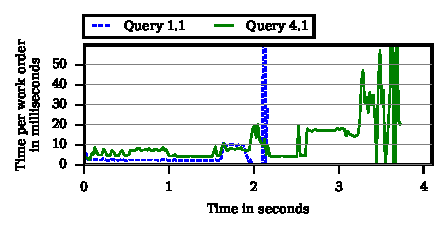
\includegraphics[width=\columnwidth]{figures/q11-q41-time-per-wo.pdf}
	\vspace{-2.5em}
	\caption{Time per work order for Q1.1 and Q4.1}
	\label{fig:q1.1-q4.1-time-per-wo}
%	\vspace{-2em}
\end{figure}

Now we analyze the execution pattern for $Q4.1$ which has 4 join operations. 
This query is more complex than $Q1.1$.% which has a single join.
%Due to the more complex nature of the query, 
Therefore, the execution pattern of $Q4.1$ exhibits more phases, with different times per work order as compared to $Q1.1$.
Various small phases before the 0.5 s mark correspond to the selection predicates that are applied to the dimension tables. (Note that in $Q4.1$ there is no selection filter on the \textit{lineorder} table).
The selections on dimension tables get executed quickly.
The longer phases denote the different probe hash table operations in the query.
Towards the end, similar to $Q1.1$, there is a spike in the execution time per work order which correspond to the aggregation phase.

It is clear that the work order execution times for both queries are different, and the difference between them changes over time. 
If the scheduler assigns the same probability to both queries (i.e. 0.5), it is equally likely to schedule a work order from either of them. 
As a result, the queries will have different CPU utilization times in a given epoch, thus resulting in an unfair CPU allocation. 
In order to be consistently fair in allocating CPU resources to the queries, we should continuously observe the work order execution times of queries and adjust the CPU allocation accordingly. % update the predicted work order execution times. 
%Later, we substantiate this explanation by an experiment (c.f. Section~\ref{ssec:learning-impact}).

In general, the time per work order metric doesn't stay the same throughout a query's lifetime.
In each phase of the query, the time per work order is different.
As the query plan gets bigger, the number of phases in the plan increase.
In addition, different queries may be in different phases at a given point in time.
To make things more complicated, queries can enter or leave the system at any time.

%$Q4.1$, the execution exhibits different ``phases'', each belonging to different relational operators in the query such as selection, building the hash table, probing the hash table, aggregation etc. 
%\reminder{Describe in the figure the begin and end times of various phases}

Therefore it is difficult to statically pick a proportion of CPU to allocate to the concurrent queries. 
Hence there is a need to ``learn'' the various phases in the query execution and dynamically change the proportion of resources allocated to each query, based on each query's phase.
Next, we study the methodology used by the Learning Agent.
\subsubsection{Learning Agent Methodology}
%The Learning Agent builds each query's \textit{execution profile} based 
%on the execution statistics of recently completed work orders for that query.
The Learning agent uses the execution times of previously executed work orders 
denoted as $t_{w_{1}}, t_{w_{2}}, \ldots, t_{w_{k}}$ to predict the execution time of 
the next work order $t_{w_{k+1}}$ for a given query.\footnote{In the beginning of a query execution, when enough information about work order execution times is not available, we use the default probabilities in the Policy Enforcer, instead of using default predicted times in the Learning Agent.}
Figure~\ref{fig:scheduler-cycle} shows the Learning Agent's interaction with the other scheduler components.
%It receives the execution statistics of an  executed work order, and uses this information 
%to predict the execution time of the future work orders. 

\begin{figure}[h]
	\centering
	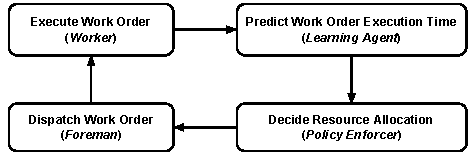
\includegraphics[width=\linewidth]{figures/Compact-SchedulerCycle.pdf}
	\vspace{-2em}
	\caption{Interactions among scheduler components}
	\label{fig:scheduler-cycle}
%	\vspace{-1.5em}
\end{figure}

The set of previously executed work orders can belong to multiple relational operators in the query operator DAG. 
The Learning Agent stores the execution times of the work orders grouped by their source relational operator, e.g. the execution statistics of select work orders are maintained together and kept separate from aggregation work orders. 

%A prediction model is used to estimate the execution time of future work orders. 
\sys{}'s scheduler currently uses linear regression as the prediction model.
We chose linear regression as it is fast, accurate, and efficient w.r.t. the computational and the memory storage overheads of the model. 
%(New models can be easily added using an abstraction mechanism.) 
To lower the CPU and memory overhead of the model, we limit the amount of execution statistics stored in the Learning Agent.
We discard records beyond a certain time window. 
When all the work orders of an operator finish execution, we remove its records completely. 
In a query, when multiple relational operators are active, 
linear regression combines the statistics of all active operators and predicts a single 
value for the next work order execution time.
%There are few reasons for the choice of our prediction methodology: We want a fast 
%technique so that the prediction itself doesn't become a  bottleneck in the core 
%execution 
%of the queries. The prediction method should be simple and reasonably accurate. The 
%linear regression approach is inexpensive and straightforward to reason about. It reacts 
%quickly and adapts well to the change of operators (and corresponding change in 
%execution times of work orders) that happen during the DAG traversal described in 
%Algorithm~\ref{alg:dag-traversal}.

We note that the problem of estimating the query execution time is well-studied 
~\cite{duggan2011performance, wu2013towards, li2012gslpi, 
chaudhuri2004estimating}. 
The Learning Agent does not require such methods. 
However, it can combine estimates from other methods with its simple learning-based estimates.
%i.e. we try to predict the execution times of immediate work orders, as opposed  to a 
%global
%level estimation that may involve estimation of the progress of the query and prediction
%of query/workload completion times. The Learning Agent can be extended to use
%other techniques for the prediction, and is complimentary to other methods for
%estimation.